\section{Geometrie- und Werkzeugkette}
\label{sec:werkzeugkette}

Die Zahnkontur für das FE-Netz des Rades und die Prüfmaße der Prüfräder werden mit einer eigenen Geometriekette aus einem Datensatz abgeleitet. Rechengrundlage sind die gültigen Normen. DIN ISO 21771 mit Anhang NB gilt für Geometrie und Erzeugung \cite{DINISO21771}, DIN 21773 für die Prüfmaße \cite{DIN21773}, DIN 867 für das Bezugsprofil \cite{DIN867} und DIN 3972 für die Werkzeug-Bezugsprofile \cite{DIN3972}. STplus rechnet die Geometrie dagegen nach der zurückgezogenen DIN 3960 von 1987 \cite{DIN3960}. Wo die Normenkette von STplus von der aktuellen Norm abweicht, ist die Abweichung mit beiden Gleichungen und einem Zahlenbeispiel in \secref{sec:anhang_b} festgehalten.

Erzeugt wird die Zahnkontur mit einem zahnstangenförmigen Werkzeug nach Abschnitt 7 der DIN ISO 21771, für Gerad- und Schrägverzahnung. Eingaben sind das Werkzeug-Bezugsprofil mit $h_{\mathrm{aP0}}$, $\rho_{\mathrm{aP0}}$, Fußformhöhe und gegebenenfalls Kantenbrechflanke, die Kopfkreisdurchmesser beider Räder und zwei der drei Werte $a_{\mathrm{w}}$, $x_1$ und $x_2$. Schrägungswinkel, Kopfkantenbruch, Protuberanz und Bearbeitungszugabe werden ausdrücklich angegeben, auch wenn sie null sind. Ausgewertet wird die Erzeugung mit dem Faktor $x_{\mathrm{Es}}$ des oberen Zahndickenabmaßes, wie STplus ihn druckt. Ein Zahn besteht aus der Fußkurve der Werkzeug-Kopfrundung bis zum Fußformkreis, der Evolvente bis zum Kopf-Formkreis, dem Kopfkantenbruch und dem Kopfkreis. Der Kantenbruch folgt aus der Kantenbrechflanke des Werkzeugs nach DIN 3960 Anhang A.3.1 \cite[S.~14]{DIN3960} oder aus den Eingaben $h_{\mathrm{K}}$ und $s_{\mathrm{aK}}$. Da keine Norm die Fußkurve geschlossen angibt, wird die Hüllbedingung des Verzahnungsgesetzes nach Linke \cite{Lin10} und FVA 604 I \cite{FVA604-I} auf das Werkzeugprofil im Stirnschnitt angewendet. Dort ist die Kopfrundung eines schrägverzahnten Werkzeugs eine Ellipse mit den Halbachsen $\rho_{\mathrm{aP0}}/\cos\beta$ und $\rho_{\mathrm{aP0}}$. Der Fußformkreis $d_{\mathrm{Ff}}$ folgt aus Gleichung (128) in der Fassung des Anhangs NB. Unterhalb der Unterschnittgrenze nach Gleichung (135) wird er als Schnittpunkt von Fußkurve und Evolvente numerisch bestimmt.

Der Abgleich mit STplus 11.1F erfolgt über ein eigenes Stapelskript. Es ruft das installierte Programm mit variierten Eingabedateien auf und liest die Ergebnislisten, die Schnittstellendatei und den Export der Stirnschnittkontur ein. Neben 18 Vergleichsfällen, darunter die Prüfverzahnung kst-E, wurden 70 Probeläufe mit unvollständigen und widersprüchlichen Eingaben gerechnet, mit denen Vorbelegungen und Grenzen des Programms an Randfällen untersucht wurden. Ein Einleseprogramm für die STplus-Eingabedateien wendet diese Vorbelegungen an und vermerkt jede einzelne \cite{STplus11-1F}. Da STplus in einfacher Genauigkeit rechnet, räumt der Vergleich jedem Wert die Rundung seiner letzten gedruckten Stelle und die 32-Bit-Arithmetik ein. In den 18 Vergleichsfällen wurden 855 Einzelwerte der Paargeometrie verglichen. Davon stimmen 786 in den gedruckten Stellen überein, 69 weichen nur im Rahmen der Genauigkeit von STplus ab. Die 533 Einzelwerte der Erzeugung zeigen dasselbe Bild. Exportierte Konturen von 28 Rädern mit Schrägungswinkeln bis $30$°, vier davon unterschnitten, weichen an der Fußkurve höchstens $0{,}6$\,µm und an der Evolvente $0{,}25$\,µm von der eigenen Kontur ab.

Nach DIN 21773 werden die Prüfmaße berechnet, die Grenzmaße nach Abschnitt 4 der Norm mit $x_{\mathrm{Es}}$, $x_{\mathrm{Em}}$ und $x_{\mathrm{Ei}}$ in den Gleichungen des Nennmaßes. Ein eingegebenes Prüfmaß nennt, ob es Nennmaß, oberes, mittleres oder unteres Grenzmaß ist. STplus liest jedes Prüfmaß als Maß der Fertigverzahnung beim oberen Abmaß. Die Messzähnezahl $k$ folgt aus Gleichung (9) der Norm, der Messkugeldurchmesser $D_{\mathrm{M}}$ als nächstgrößerer Wert der DIN 3977 \cite[Tabelle 1, S.~2]{DIN3977} über dem idealen Durchmesser nach Gleichung (26). STplus wählt beide nach Regeln, die das Handbuch nicht nennt. Diese Regeln wurden gefunden, indem die Eingaben schrittweise bis zu den Werten verändert wurden, an denen STplus von einem $k$ oder $D_{\mathrm{M}}$ zum nächsten wechselt. Mit 540 zufällig erzeugten Rädern wurden sie ohne Abweichung bestätigt. Das Einleseprogramm führt die Regeln von STplus neben der Normregel und vermerkt bei jedem Wert, welche von beiden angewendet wurde.

% TK erledigt (Zähler erklärt: 18 Fälle + 70 Probeläufe = STplus-Läufe; 855/533 = Einzelwerte darin; 540 Zufallsräder = Prüfung der Prüfmaßregeln): der satz endet und stehen benannt neben der Normregel. Der Leser weiß nicht, was damit gemeint ist. Versetze dich beim schriben mehr in eine Person, die nicht so tief in den Aufbau des Programms drin steckt. Und die Zahlen sind für den Leser etwas aus der Luft gegriffen. Oben sind es noch 533 Vergleiche, jetzt 540 Zufallsräder, dann mal 18 Vergleichsfälle und 70 Probeläufe. Bitte präzisieren, was wirklich gemeint ist.

Für die Untersuchung der Fußgeometrie in \secref{sec:fussgeometrie} ersetzt eine Variante die Trochoide der Werkzeug-Kopfrundung zwischen einem Übergangsdurchmesser auf der Flanke und der Lückenmitte. Oberhalb des Übergangs bleibt die Kontur die der Erzeugung, das Ritzel bleibt unverändert. Jede Kurve schließt tangentenstetig an die Flanke an und kreuzt die Lückenmitte im rechten Winkel. Der Fußkreis der Variante geht durch diesen Punkt. Nach Frühe \cite{Frue12} beginnt die geneigte Ellipse am Fußformkreis und wird durch den Neigungswinkel $\gamma$ und das Achsenverhältnis $a/b$ bestimmt. Die kubische Bézierkontur nach DE 10 2013 004 861 B3 \cite{DE102013004861B3} legt ihre Kontrollpunkte auf die Flankentangenten im Abstand $(0{,}25 + 0{,}1 f)\,l$ vom Flankenpunkt. Die Bernstein-Form stammt von Roth und Opferkuch \cite{RotOpf17}. Bei der bionischen Kontur nach DE 10 2008 045 318 B3 führt eine Tangensfunktion vom Flankenpunkt zu einem Kreis vom Radius $r$ auf der Lückenmitte, der den Fußkreis berührt. Der Flankenwinkel $\varphi$ folgt aus Anspruch 5 \cite{DE102008045318B3}. Beide Patentkonturen setzen am maßgebenden Durchmesser $d_{\mathrm{r}} = (d_{\mathrm{N}} + d_{\mathrm{FR}})/2$ an, zwischen dem Beginn des nutzbaren Profils und dem tiefsten Kreis, den der Ritzelkopf erreicht. Das Wachstumsverfahren nach Kassem \cite{Kas23} liefert keine geschlossene Kurve und bleibt außen vor. Kinematisch geprüft wird jede Variante, indem die Kopfkanten der Ritzelzähne mit der Wälzbewegung durch die Lücke geführt werden. Unterschreitet ihr kleinster Abstand zur Fußkurve $0{,}02$\,mm, wird keine Eingabedatei geschrieben. Die Netzvorlage des Sektors legt sich unverändert auf die neue Kontur. Zur Vorauswahl der Parameter diente eine ebene Studie am Sektor mit drei Zähnen unter W1 bei $16$\,Nm mit Lastfleck am Normpunkt B. Sie umfasste 42 Ellipsen, 7 Bézierkonturen und 36 bionische Konturen. \figref{fig:fussrundungsvarianten} zeigt die sechs gerechneten Konturen gegen die Trochoide.

\begin{figure}[htbp]
    \centering
    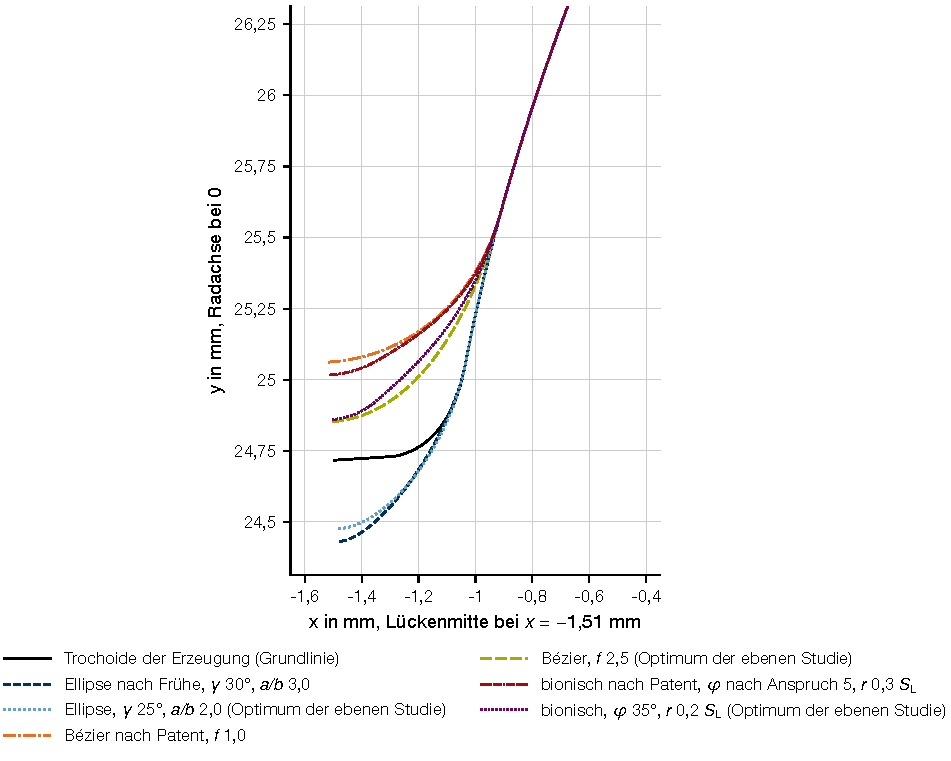
\includegraphics[width=0.85\textwidth]{kap3/fussrundungsvarianten}
    \caption{Fußrundungsvarianten des Rades kst-E im Stirnschnitt gegen die Trochoide der Erzeugung, linke Zahnhälfte von der Lückenmitte bis zur Evolvente. Die Ellipsen setzen am Fußformkreis an, die Patentkonturen am maßgebenden Durchmesser $d_{\mathrm{r}}$.}
    \label{fig:fussrundungsvarianten}
\end{figure}

Die Programme der Geometriekette, die Abaqus-Eingabedateien, die Datenauswertung und der Bildbau wurden in Python mit KI-gestützter Programmierung erstellt (Claude Code, Modell Fable 5.1). Zu jeder Rechenfunktion ist die Gleichung ihrer Quelle mit Ausgabe und Fundstelle vermerkt. Gerechnet wird durchgehend in doppelter Genauigkeit ohne Rundung innerhalb der Kette. Als pydantic-Modelle mit Prüfregeln sind die Datenstrukturen der Kette beschrieben, etwa für Wertebereiche und für die Reihenfolge der Durchmesser $d_{\mathrm{b}} \le d_{\mathrm{Ff}} < d_{\mathrm{Fa}} \le d_{\mathrm{a}}$. Eine fehlende Angabe wird gemeldet statt vorbelegt. Diese Beschreibung der Daten leitet zum Ausblick über, in dem Datenverträge für die Messprotokolle und die Rohdaten des Labors vorgeschlagen werden (\secref{sec:ausblick}).

% Bildwunsch: Konturvergleich gearcore gegen STplus (Zahnkontur-Export) / Konturen der drei Fußrundungsvarianten gegen die Trochoide
% (Labels im Text: fig:konturvergleich_stplus, fig:fussrundungsvarianten; noch nicht in bilder.yaml).

% Herkunft:
% Absatz 1 (Zweck, Normen): architecture_decisions.md ADR-105 Z. 137 bis 150 (aktuelle Norm gilt, DIN 3960
%   zurückgezogen, Abweichungen mit beiden Gleichungen und Zahlenbeispiel); norm_map.md Z. 8 bis 23 (Zuordnung
%   DIN 3960 → DIN ISO 21771, DIN 21773, DIN ISO 1328-1; DIN 867, DIN 3972).
% Absatz 2 (Erzeugung, Kontur): ADR-110 Z. 386 bis 393 (zwei von a_w, x_1, x_2; Kopfkreis ist Eingabe); ADR-111
%   Z. 517 bis 522 (Null wird angegeben); ADR-113 Z. 597 bis 620 (x_Es, Gl. (128) NB, Gl. (135), Schnittpunkt
%   numerisch, Hüllbedingung nach Linke und FVA 604 I, Ellipse der Kopfrundung) und Z. 621 bis 629 (Kantenbruch nach
%   DIN 3960 A.3.1 oder h_K und s_aK); contour.py Modul-Docstring Z. 1 bis 17 (Aufbau des Zahnes); norm_map.md
%   Z. 35 bis 37 (keine Norm gibt die Trochoide geschlossen an).
% Absatz 3 (Abgleich mit STplus): ADR-102 Z. 54 bis 66, Z. 85 bis 90 und Z. 97 (Stapelbetrieb, Konturexport,
%   Schnittstellendatei); ADR-106 Z. 165 bis 181 (einfache Genauigkeit, Toleranzen des Vergleichs); ADR-110
%   Z. 455 bis 457 (18 Fälle, 855 Vergleiche: 786 / 69 / 0); ADR-113 Z. 650 bis 651 und Z. 663 bis 665
%   (533 Vergleiche: 364 / 169 / 0; Konturen 0,6 / 0,25 µm, 14 Läufe, 28 Räder, vier unterschnitten, β bis 30°);
%   ADR-114 Z. 683 bis 686 und Z. 698 bis 702 (70 Probeläufe, Importer wendet Vorbelegungen an und vermerkt sie).
% Absatz 4 (Prüfmaße): ADR-115 Z. 856 bis 863 (DIN 21773, DIN 3977, STplus liest Prüfmaß als oberes Abmaß), Z. 867 bis
%   870 (Art des Maßes), Z. 876 bis 878 (Grenzmaße nach §4 mit x_Es, x_Em, x_Ei), Z. 879 bis 884 (k nach Gl. (9);
%   D_M aus DIN 3977 Tabelle 1 über Gl. (26), (27)), Z. 885 bis 896 (Regeln von STplus durch Bisektion der
%   Umschaltpunkte gefunden, 540 Zufallsräder, benannt, nie stillschweigend).
% Absatz 5 (Fußrundungsvarianten): ADR-116 Punkt 52 Z. 1793 bis 1822 (Konturersatz zwischen Übergang und Lückenmitte,
%   Ellipse nach Frühe Abschnitt 5.4.1 mit γ und a/b, Bézier nach DE 10 2013 004 861 B3 Anspruch 8 mit
%   k = (0,25 + 0,1 f) l und Bernstein-Form nach Roth und Opferkuch, bionisch nach DE 10 2008 045 318 B3 mit Tangens-
%   funktion, Kreis r, φ nach Anspruch 5, Übergang bei d_Ff bzw. d_r = (d_N + d_FR)/2, kinematische Prüfung, 0,02 mm,
%   Netzvorlage unverändert), Z. 1835 bis 1837 (Kassem 2023 bleibt außen vor), Z. 1846 bis 1851 (ebene Studie: drei
%   Zähne, eigener Löser, W1 16 Nm, Lastfleck an B, 42 / 7 / 36 Varianten); fillet.py Modul-Docstring Z. 1 bis 25,
%   Z. 235 bis 238 (l als Abstand des Hauptpunkts vom Tangentenschnittpunkt), Z. 340 bis 341 (d_FR als tiefster
%   Durchmesser, den der Gegenradkopf erreicht).
% Absatz 6 (Umsetzung): 00_schreibregeln.md Abschnitt 2 Punkt 3 (Nennung der KI-gestützten Programmierung, pydantic,
%   Ausblick); gearcore README.md Z. 3 und Z. 13 bis 14 (pydantic-Datenverträge, jede Rechenfunktion nennt Quelle und
%   Gleichung); ADR-106 Z. 171 bis 175 (doppelte Genauigkeit ohne Rundung in der Kette); ADR-110 Z. 413 bis 422
%   (Prüfregeln: Typen, Wertebereiche, d_b ≤ d_Ff < d_Fa ≤ d_a); norm_map.md Z. 297 bis 300 (fehlender Wert wird
%   gemeldet, keine stillen Vorbelegungen).
% Zitate: ISO14 = DIN ISO 21771 (2014), DIN14 = DIN 21773 (2014), DIN86 = DIN 867 (1986), Lin10 = Linke 2010,
%   Frue12 = Frühe 2012 (Schlüssel in der Bib: Frü12). Rot17 ist FVA 732 I (Roth Z.), nicht Roth und Opferkuch 2017
%   (VDI-Berichte 2294): deshalb Platzhalter. Keine Bib-Einträge für DIN 3972, FVA 604 I, STplus-Programmanleitung,
%   die beiden Patente und Kassem 2023 (Zim16 ist FVA 604 II).
